% Chapter Template

\chapter{Option Pricing And Deep Learning} % Main chapter title

\label{Chapter5} % Change X to a consecutive number; for referencing this chapter elsewhere, use \ref{ChapterX}

Deep learning can be applied to option valuation in different ways. After the two sections with MLPs calibrated to pricing models the MLPs will be applied to approximate optimal exercise strategy similar to LSM. The second method is to simulate input parameter, i.e. the market parameters and model parameters and then using a classical method for calculating target values $\bm{y}$ for the given input parameters $\matr{X}$. The method falls within supervised regression where we will use a MLPs network introduced in section \ref{multilayerPerceptron} to approximate the mapping. The risky assets are modelled with black scholes theory from earlier chapters hence the generations of labels for european and american stock options are already presented (Chapter \ref{Chapter2}, \ref{Chapter3}). The theory in chapter \ref{Chapter4} will be specialized for the specific task and discussed. The supervised MLPs regression will be used to valuate european call options and american put options. The advantage of MLPs is the model can easily be extendend to high dimensional data, where the e.g. polynomial regression (section \ref{LSM}) is prone to overfit and slow compared to MLPs. 

%----------------------------------------------------------------------------------------
%	SECTION 1
%----------------------------------------------------------------------------------------
\section{Multilayer Perceptrons Regression For Optimal Stopping}


%----------------------------------------------------------------------------------------
%	SECTION 2
%----------------------------------------------------------------------------------------
Universal approximate theorem

\section{Multilayer Perceptrons Regression Pricing From Existing Methods}
The MLPs pricing method has a different approach than the other methods, because it is only data drivin in the sense it is model free. The MLPs could easily be used to real data, which is investigated in \parencite{GasparRaquel20}. We revisit the work from \parencite{HirsaAli2019}, where we try to extend the pricing models to options with two underlying risky assets. The model will be the classical GBM model presented in earlier chapters. By choosing the GBM model the MLPs pricing method is ready for investigation both for vanilla options and exotic options. We stress that the MLPs pricing method is not restricted to GBM assumption, but can be applied to other models such as Hesten, Variance Gamma and real market data. The advantages with MLPs are the fast calibration and parameter estimation compared to classical methods binomial lattice and LSM. With the increased speed for pricing it can cost accurary specially if the data is sparse, which can arise when using the method for exotic options on real market data. For practical application the accuracy is severe if the predicted price is not within the bid-ask spread, because the aim is to price fast without introducing arbitrage. We will present results for european, american and other exotic options presented in earliar chapters with MLPs pricing methods.\\

For deep learning the hyperparameters is important for finding the right model for pricing, where different choices will be empirical presented under training. For the given task polynomial regression can also be used, but we will see later why MLPs regression is preferred. The section is split into three sections "Data", "Training" and "Performance", where the european call, american put, european put minimum and american put minimum option will be presented.

%-----------------------------------
%	SUBSECTION 1
%-----------------------------------
\subsection{Data}
The generation of labels are the computational expensive part of the MLPs method, because the method needs enough samples to approximate the function $f^*$ well. The upside after generation of labels is that the method is computationally fast and easy to implement with basic knowledge of deep learning. The labels will be generated by existing methods presented in chapter \ref{Chapter3}, where the input parameters will be quasi sampled with halton sequences.\\

For both the european call and the american put the parameter in-sample will be the same, where we remember the 5 parameters for pricing an european call option (proposition \ref{BS-price-EuroCall}). The european call and american put option is a first order homogeneous function in $(S(0),K)$, hence the valuation formula can be modified:
$$\frac{c(S(0),K)}{K}=c(\frac{S(0)}{K},1) \quad and \quad \frac{P(S(0),K)}{K}=P(\frac{S(0)}{K},1)$$
The alternative representation above reduces the number of parameters needed for simulation to 4, because instead of simulate both $S$ and $K$, moneyness ($\frac{S(0)}{K}$) is only  simulated. The input matrix $\matr{X}$ is different combinations of the 4 parameters within the parameter range (table \ref{tab:vanillaParRange}), where it is assumed the number of trading days are 252 in a year. The other parameter ranges are moneyness between 0.8 and 1.2, risk free rate of return between 1-3 \% and volatility between 0.05 and 0.5. 

\begin{table}[H]
\caption[Parameter Ranges For MLPs]{Parameter ranges for american put and european call options}
\label{tab:vanillaParRange}
\centering
\begin{tabular}{l l l l l}
\toprule
\textbf{Derivative} & \textbf{r} & \textbf{T} & \textbf{Moneyness} & $\sigma$ \\
\midrule
Euro. Call & 1\%-3\% & 1d - 3y & 0.8-1.2 & 0.05-0.5\\ 
Amer. Put & 1\%-3\% & 1d - 3y & 0.8-1.2 & 0.05-0.5\\ 
\bottomrule\\
\end{tabular}
\end{table}

The european put minimum and american put minimum option for two underlyings will require additional parameters, because now we have two spots, two volatilities and correlation between the assets. The first order homegeneity does not hold for multivariate contingent claims, hence the strike and the two spots are also needed. The parameters considered for the bivariate contingent claims are T, r, K, $S_1(0)$, $S_2(0)$, $\sigma_1$, $\sigma_2$ and $\rho$ so a total of 8 parameters, and the given parameters ranges are given in table \ref{tab:ExoticParRange}.
   
\begin{table}[H]
\caption[Parameter Ranges For MLPs]{Parameter ranges for exotic european put and american put options}
\label{tab:ExoticParRange}
\centering
\begin{tabular}{l l l l l l l l l l l}
\toprule
\textbf{Derivative} & \textbf{r} & \textbf{T} & K & $S_1(0)$ & $S_2(0)$ & $\sigma_1$ & $\sigma_2$ & $\rho$ \\
\midrule
Euro. Put Min. & 1\%-3\% & 1d - 3y & 80-120 & 100 & 100 & 0.05-0.5 & 0.05-0.5 & 0.05-0.5\\ 
Amer. Put Min. & 1\%-3\% & 1d - 3y & 80-120 & 100 & 100 & 0.05-0.5 & 0.05-0.5 & 0.05-0.5\\
\bottomrule\\
\end{tabular}
\end{table}

The simulationen of the parameter ranges is done by quasi-random Halton sequences sampling instead of e.g. random sampling like uniform sampling to obtain lower discrepancy. The Halton sequence covers the space more evenly quicker, because of the lower discrepancy. Like uniform sampling the halton sequence points is between 0 and 1, hence we need to apply a transformation to get the parameter ranges:
$$r \cdot (range \ of \ parameter) + lowerBound \quad where \ r=halton \ point$$
After the simulation of combinations of the input parameters within the given ranges the labels can be generated from existing methods. For the european call option the generation of labels is done by the classical B-S formula for call options given in proposition \ref{BS-price-EuroCall}. The B-S pricing formula is well known and has an analytical solution, hence it is relatively fast to generate labels in this model. In the B-S setup in section \ref{classicBS} we assume constant volatility, which is not realistic in terms of the known fact that volatility skew for equity options (p. 458 \parencite{Hull}). The european put minimum option is by the change of numeraire method given in closed form in section \ref{BMHiggerDim}, hence the generation of labels like in the B-S price formula is fast. The american options require numerical methods, hence the generation of labels are more computational expensive. The labels for the american options are generated by CRR for american put option with 1 underlying stock and by BEG for two underlyings presented in chapter \ref{Chapter3}. When the datasets ($\matr{X}$, $\bm{y}$) are generated we are left with a regression task. The regression task is to predict the price $\bm{y}$ from the input parameters $\matr{X}$.\\ 

The datasets generated for training the model will be the in-sample data set, where the parameters are sampled within the parameter ranges for the given derivative. The in-sample dataset are split up into a training and validation dataset in order to measure model performance. The training dataset is used to update the parameters weights,biases, etc. internal in the model and finetune hyperparameters for choosing the optimal model design. To avoid overfitting and good generalization models the validation set is useful, because the trained model has not seen the data before evaluation on validation set. The validation set is randomly subsampled from the training set, where the validation dataset constitute 20 procent of the training set. To check the robustness of the regression we choose to sample two test datasets out-of-sample, which means we simulate data with modified parameter ranges. \\

The test datasets out-of-sample is simulated by adjusting the parameter range for either moneyness or maturity for the options with 1 underlying. For the options with two underlyings the parameter ranges for the spot and the maturity is modified for the out-of-sample test sets. The test dataset has not been seen by the model in the training process, hence we get a unbiased evaluation of the model. The aim with producing different test and validation data sets is to measure the models performance at interpolation and extrapolation. We have illustrated the marginal distributions for the american put option with a training dataset of 300.000 samples. The marginal distributions (figure \ref{fig:marginalAmerPut}) shows that we have succesfully generated parameters in the given ranges and the parameters are evenly spaced in the ranges. 
 
\begin{figure}[H]
\centering
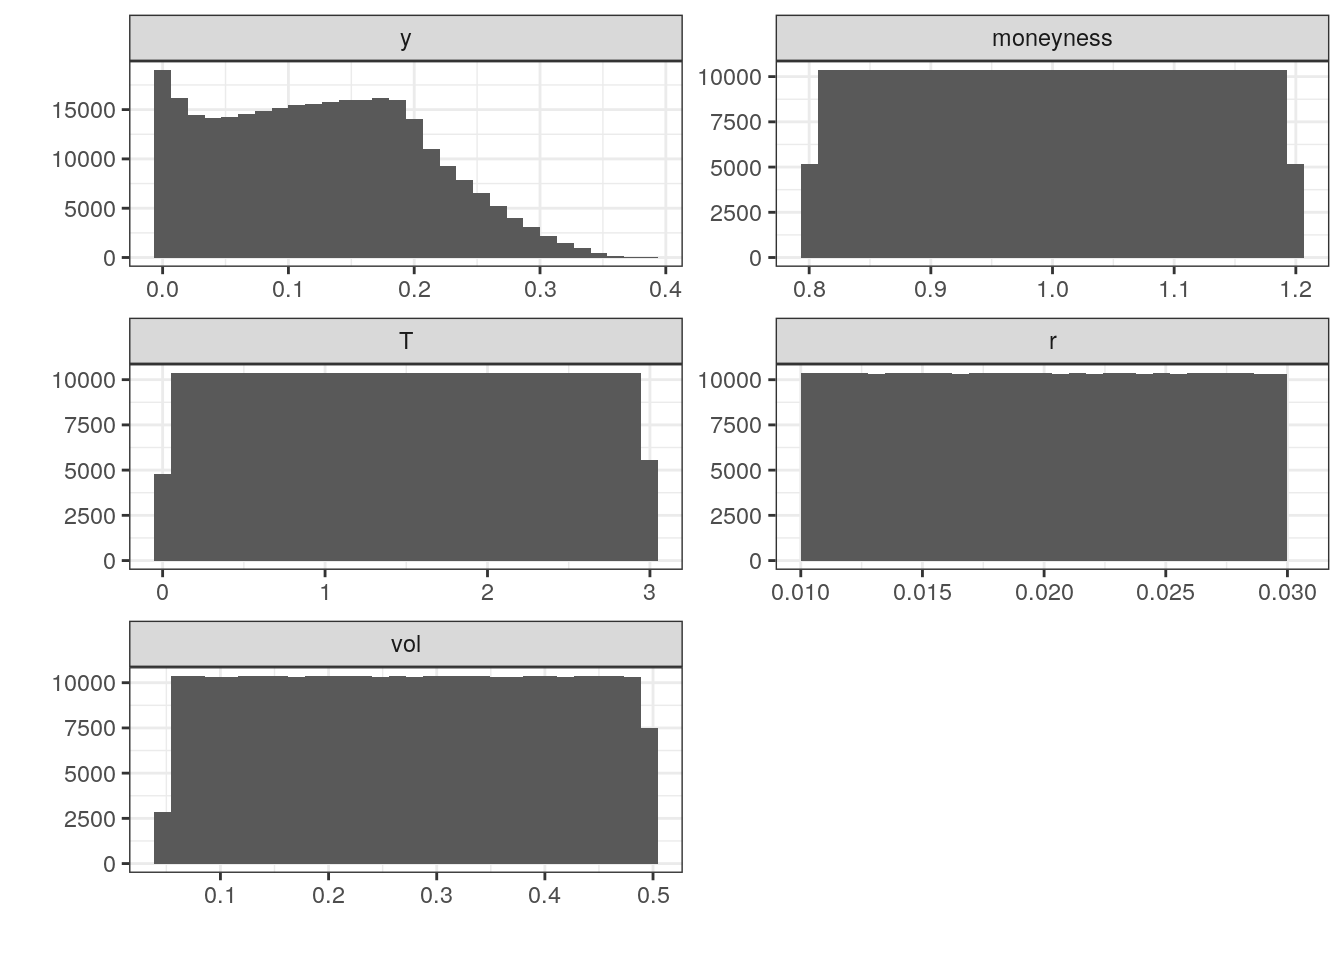
\includegraphics{Figures/marginalAmerPut.png}
\decoRule
\caption[Marginal Distributions For American Put]{Quasi random simulation with halton sequence for input variables and CRR for generation of labels for american put option.}
\label{fig:marginalAmerPut}
\end{figure}
The marginal distributions shown is for $300.000$ data samples ($\matr{X},y$) generated by halton sequences and CRR model, where the marginal distributions for the features cover the parameter range almost uniform and the simulated y lies with most values at zero and maximum at 0.387 rounded to three decimals. In the model performance section out-of-sample dataset will be used to check the predictive strength of the models. The out-of-sample test dataset will be 60.000 generated with halton sequences sampling like the in-sample dataset and the parameter ranges for the options with 1 underlying is given in \ref{tab:totalVanillaParRange}.

\begin{table}[H]
\caption{Parameter ranges for european call and american put option}
\label{tab:totalVanillaParRange}
\centering
\begin{tabular}{l l l l l l l l }
\toprule
\textbf{Dataset} & Derivative &\textbf{Moneyness} & \textbf{r} & \textbf{$\sigma$} & \textbf{T} \\
\midrule
In-Sample & Euro. Call & 0.8-1.2 & 1\%-3\% & 0.05-0.5 & 1d-3y\\ 
Out-Of-Money & & 0.6-0.8 & 1\%-3\% & 0.05-0.5 & 1d-3y\\ 
Longer Maturity & & 0.8-1.2 & 1\%-3\% & 0.05-0.5 & 3y-5y\\ 
In-Sample & Amer. Put & 0.8-1.2 & 1\%-3\% & 0.05-0.5 & 1d-3y\\ 
Out-Of-Money & & 1.2-1.4 & 1\%-3\% & 0.05-0.5 & 1d-3y\\ 
Longer Maturity & & 0.8-1.2 & 1\%-3\% & 0.05-0.5 & 3y-5y\\ 
\bottomrule\\
\end{tabular}
\end{table}
The out-of-sample for the multivariate contigent claims will be similar, except that the strike will be between 120-140, because first order homegeneity does not hold for the multivariate contingent claims.

%\begin{figure}[H]
%\centering
%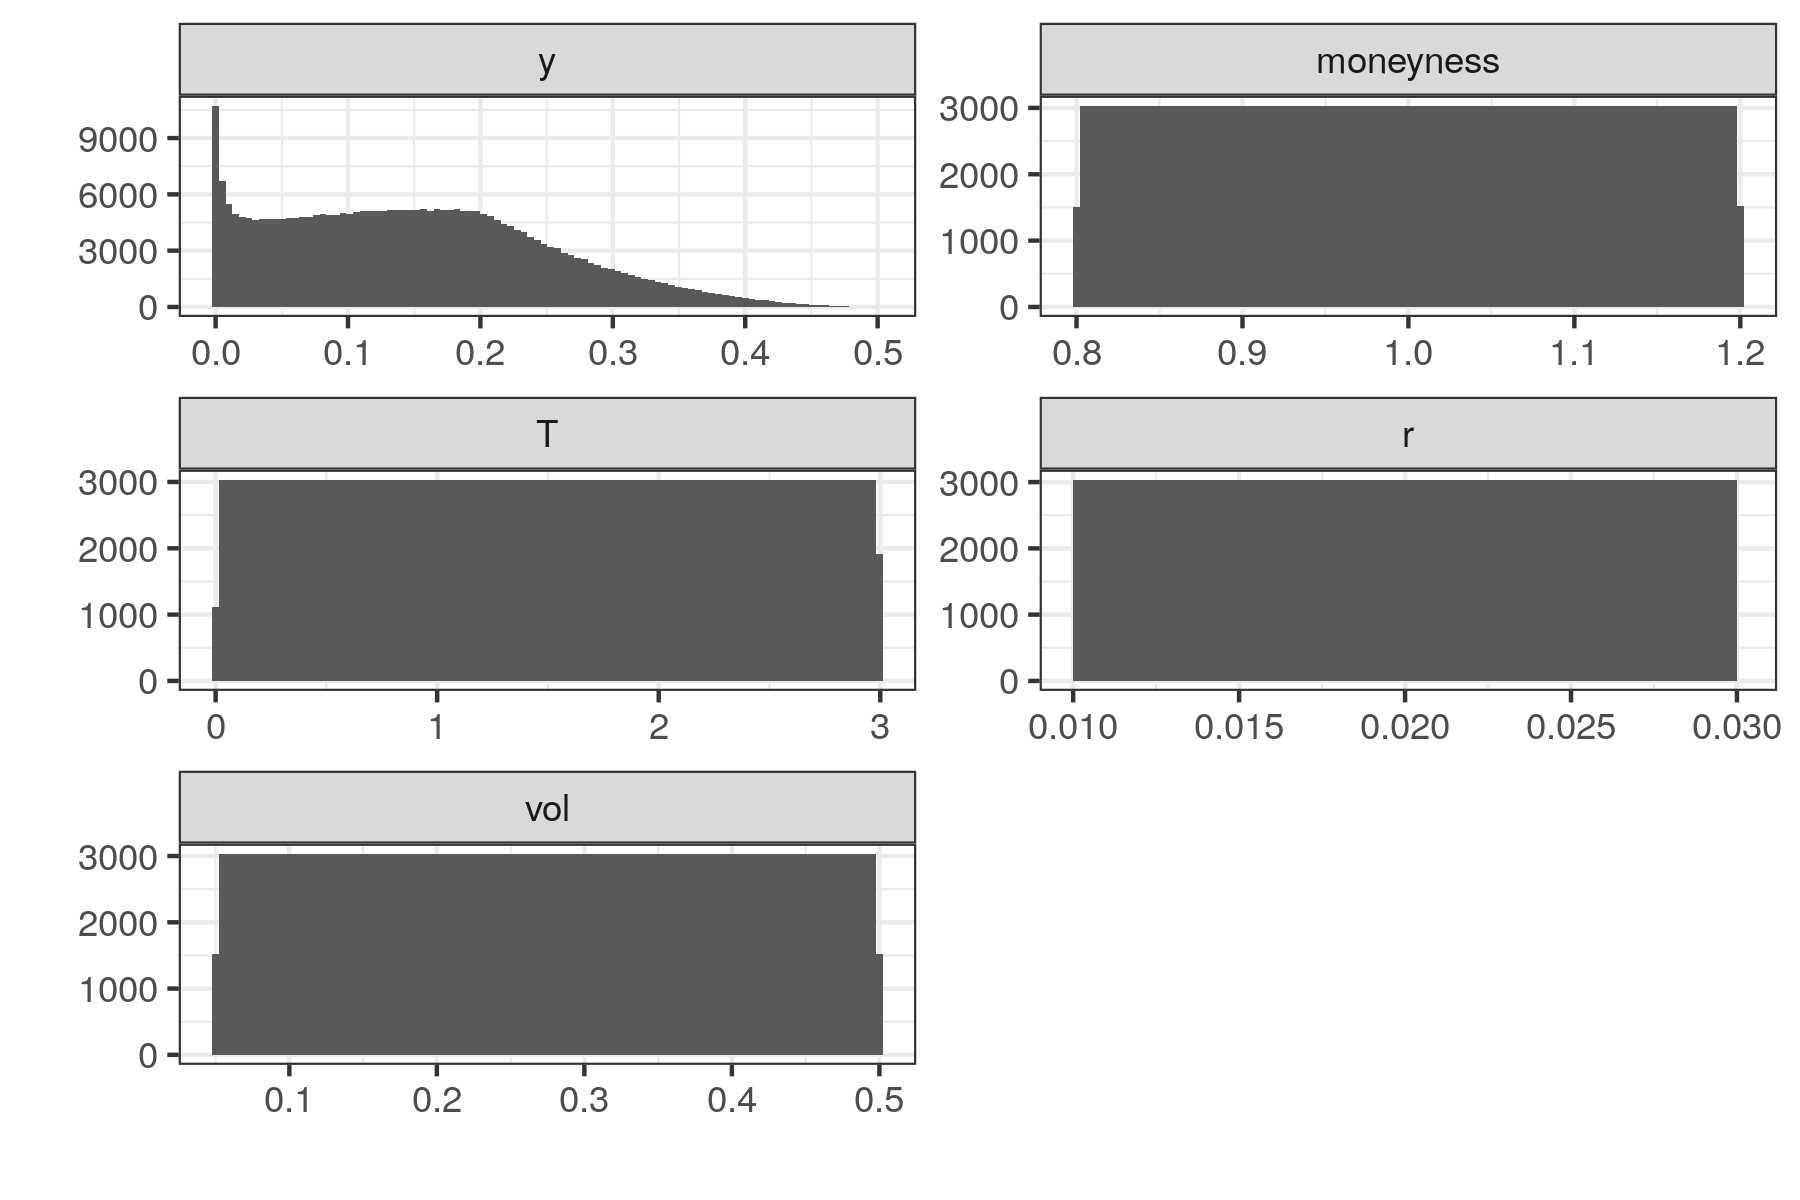
\includegraphics{Figures/marginalEuroCall.png}
%\decoRule
%\caption[Marginal distributions for european call]{Quasi random simulation with halton sequence}
%\label{fig:marginalEuro}
%\end{figure}

%-----------------------------------
%	SUBSECTION 2
%-----------------------------------

\subsection{Training}
The in-sample data is the simulated data within the parameter ranges for the different types of derivatives, where the aim is that the model will learn the pricing function $f^*$. Once the dataset ($\matr{X}, \bm{y}$) is generated the model can be trained to approximate the true function $f^*$. To train the model we use MLPs regression to infer the pricing function from the generated data, hence the approach is model free, because the data is only needed. We will also present a standard linear model to compare the MLPs with the classical regression methods. We want to have a fast, robust and accurate model after training on the training set. To train the model we need a measure for the error, where the standard mean squared error (MSE) for regression is applied. I.e. the cost function chosen to be the empirical risk function with a quadratic loss function:
$$J(\theta)= \frac{1}{n} \sum_{i=1}^{n}(y_i-\hat{y}_i)^2$$
The MSE penalizes outliers stronger than e.g. mean absolute error (MAE), but it penalize small deviations less. To update the weights the Adam optimization algorithm is chosen with learning rate set to $\eta=0.001$, which is a standard choice for MLPs. \\

We test empirically the best hyperparameters for the MLPs, where the validation set is used. The first investigation is to look how well the model performs on varying dataset sizes, where the goal is to quantify how large datasets is needed for having a high quality model. The datasets for an european call option considered are in-sample datasets of size 100, 1K, 10K, 100K, 300k, 1M data samples, where the validation set is subsampled from the training data set. By inspiration from \parencite{HirsaAli2019} we choose to test the datasets with a MLPs with 4 layers, 120 neurons in each hidden layer and 1 output. In each layer we choose the activation function leaky ReLU, which is one of the most popular choices for activation functions. The number of data samples is relevant for real data, because for real market data there is not unlimited market data available.

\begin{figure}[H]
\centering
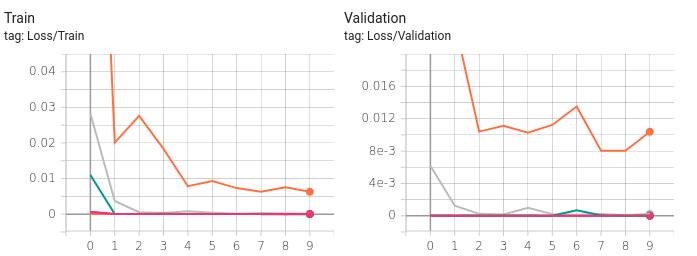
\includegraphics[width=\textwidth]{Figures/euroTestDataset.png}
\decoRule
\caption[Effect of dataset size]{Effect of gather more data on training and validation loss, where the x-axis is number of epoch-1 and y-axis is the loss for the training and validation loop. The orange line with the largest is for 100 datapoints, the grey line for 1000 datapoints, the green line 10K datapoints, the three last lines blends together where it is for 100K,300K and 1M datapoints. More can be seem at \href{https://tensorboard.dev/experiment/JURHMdo6Ra6MRW5XnlYwkg/\#scalars&run=EuroCall\%2FEuroMLP1K\&\_smoothingWeight=0\&runSelectionState=eyJFdXJvQ2FsbC9FdXJvTUxQMTAwIjp0cnVlLCJFdXJvQ2FsbC9FdXJvTUxQMTAwLzE2MDE5MjcyNTMuOTkyMTYxMyI6dHJ1ZSwiRXVyb0NhbGwvRXVyb01MUDEwMC8xNjAxOTI3MjU0LjAwODY1NTUiOnRydWUsIkV1cm9DYWxsL0V1cm9NTFAxMDAvMTYwMTkyNzI1NC4wMjYzMTA3Ijp0cnVlLCJFdXJvQ2FsbC9FdXJvTUxQMTAwLzE2MDE5MjcyNTQuMDQzODcyIjp0cnVlLCJFdXJvQ2FsbC9FdXJvTUxQMTAwLzE2MDE5MjcyNTQuMDU3NjkwNCI6dHJ1ZSwiRXVyb0NhbGwvRXVyb01MUDEwMC8xNjAxOTI3MjU0LjA2NzcyOTIiOnRydWUsIkV1cm9DYWxsL0V1cm9NTFAxMDAvMTYwMTkyNzI1NC4wODIzMDczIjp0cnVlLCJFdXJvQ2FsbC9FdXJvTUxQMTAwLzE2MDE5MjcyNTQuMDg5ODkzNiI6dHJ1ZSwiRXVyb0NhbGwvRXVyb01MUDEwMC8xNjAxOTI3MjU0LjEwMDA5ODQiOnRydWUsIkV1cm9DYWxsL0V1cm9NTFAxMDAvMTYwMTkyNzI1NC4xMTk4NSI6dHJ1ZSwiRXVyb0NhbGwvRXVyb01MUDEwMEsiOnRydWUsIkV1cm9DYWxsL0V1cm9NTFAxMEsiOnRydWUsIkV1cm9DYWxsL0V1cm9NTFAxSyI6dHJ1ZSwiRXVyb0NhbGwvRXVyb01MUDFNIjp0cnVlLCJFdXJvQ2FsbC9FdXJvTUxQMU0vMTYwMTkyNzQ4NC44MzczMjQ5Ijp0cnVlLCJFdXJvQ2FsbC9FdXJvTUxQMU0vMTYwMTkyNzUzMS42OTg0MjciOnRydWUsIkV1cm9DYWxsL0V1cm9NTFAxTS8xNjAxOTI3NTgwLjYxOTQwODQiOnRydWUsIkV1cm9DYWxsL0V1cm9NTFAxTS8xNjAxOTI3NjMxLjEwNjM5ODgiOnRydWUsIkV1cm9DYWxsL0V1cm9NTFAxTS8xNjAxOTI3Njc3LjEzMTg4MjIiOnRydWUsIkV1cm9DYWxsL0V1cm9NTFAxTS8xNjAxOTI3NzIyLjg2Nzk2ODMiOnRydWUsIkV1cm9DYWxsL0V1cm9NTFAxTS8xNjAxOTI3NzY4LjY2MDgwODYiOnRydWUsIkV1cm9DYWxsL0V1cm9NTFAxTS8xNjAxOTI3ODE0LjA0NjU0NiI6dHJ1ZSwiRXVyb0NhbGwvRXVyb01MUDFNLzE2MDE5Mjc4NTkuMDAzNzc5Ijp0cnVlLCJFdXJvQ2FsbC9FdXJvTUxQMU0vMTYwMTkyNzkwNC4xODYyODciOnRydWUsIkV1cm9DYWxsL0V1cm9NTFAzMDBLIjp0cnVlfQ\%3D\%3D}[TensorBoard EuroMLP]}
\label{fig:dataComparisonEuroMLP}
\end{figure}

From figure \ref{fig:dataComparisonEuroMLP} we see that the the model performs very well for in-sample data with only 1K datapoints, when looking closer at the tensorboard the validation error is not lower for 1M datapoints than 100K and 300K datapoints. The model is only trained once on each datasets, so there is some randomness on each run, but the picture is clear. The model to interpolate prices for european call options in-sample data does not significant improve with gathering more data than 1K-10K datapoints this is good news for using the method on real market data. In the article \parencite{GasparRaquel20} they conduct a study to price american put options with real market data, where they conclude they got better results than for LSM with around 40K datapoints which is in line with the result in figure \ref{fig:dataComparisonEuroMLP}. For our controlled setup with simulated data we can choose arbitrary many datapoints albeit making the method more computational expensive. By above discussion we choose to work with 300K datapoints i.e. the same dataset size as in \parencite{HirsaAli2019} in order to compare results, the new thing compared to \parencite{HirsaAli2019} is that we will also try to price bivariate contingent claims with the MLPs regression method. The main focus in the rest of this section is to train the model for pricing multivariate contigent claims.\\
\\


\begin{table}[H]
\caption{Performance of in-sample and out-of-sample dataset of different sizes for MLPs regression on a european call option}
\label{tab:euroDataSize}
\centering
\begin{tabular}{l l l l l l l l }
\toprule
\textbf{Model} & \textbf{Dataset} & \textbf{MSE} & \textbf{RMSE} & \textbf{MAE} & \textbf{$R^2$} \\
\midrule
MLPs & In-sample Training: 800 & 0.000092 & 0.009601 & 0.007214 & 0.989676\\
MLPs & 8K & 0.000015 & 0.003875 & 0.002999 & 0.998518\\
MLPs & 80K & 0.000008 & 0.002914 & 0.002466 & 0.999167\\
MLPs & 240K & 0.000006 & 0.002419 & 0.001966 & 0.99942\\
MLPs & 800K & 0.000004 & 0.002098 & 0.001742 & 0.999565\\
MLPs & In-sample Validation: 200 & 0.000092 & 0.009601 & 0.007214 & 0.989676\\
MLPs & 2K & 0.000015 & 0.003875 & 0.002999 & 0.998518\\
MLPs & 20K & 0.000008 & 0.002914 & 0.002466 & 0.999167\\
MLPs & 60K & 0.000006 & 0.002419 & 0.001966 & 0.99942\\
MLPs & 200K & 0.000004 & 0.002098 & 0.001742 & 0.999565\\
\bottomrule\\
\end{tabular}
\end{table}

The standard measures mean square error (MSE) and root mean square error (RMSE) shows that the MLPs increase its precision for in-sample interpolation, but for the out-of-sample datasets the decreasing error hits a plateau for 80K data samples. This 


%MLPs & Out-Of-Money: 60K & 0.000075 & 0.008656 & 0.006250 & 0.956157\\
%MLPs &  & 0.000033 & 0.005702 & 0.004084 & 0.980976\\
%MLPs &  & 0.000005 & 0.002253 & 0.001770 & 0.997031\\
%MLPs &  & 0.000005 & 0.002152 & 0.001569 & 0.997291\\
%MLPs &  & 0.000006 & 0.002371 & 0.001715 & 0.996710\\

and out-of-sample datasets with 60K samples

actual data samples agrees with the model for both in-sample and out-of-sample. The in-sample training is based on the parameter ranges in table \ref{tab:euroParRange}, where the out-of-sample is 60.000 simulated samples, where the moneyness lies between 0.6-0.8 and the other ranges remain the same.  Table \ref{tab:euroDataSize} shows how the validation error for in-sample and the test-error for out-of-sample datasets perform varying the number size of the training dataset. The validation error declines for increasing sample size, but the test error does not improve significantly for 100K up to 1M. The test error decreases for 100K-300K, but it increases for 300K-1M, hence we choose to work with the 300K dataset in the analysis. The 
RMSE match units - standard deviation of residuals how much spread away from mean
Coefficient of determinant metric of correlation
variation around the mean.
predictic how the regression does compared to only fitting with the mean
Does our regression fit better the data than the mean
less variation around the mean. Hence most variation is explained by the regression. some number less variation around the line vs the mean
agrees fits for most samples, but for 



The same architecture is applied to each dataset and the Adam optimizer uses minibatches of size 64.

The training algorithm is 


Training the model is how the mode
does not know anything about the function





 , where . The architecture of the network  where in hyperparameter tuning, we will try with elu in each layer instead. The architecture is chosen based on the investigation done in  \parencite{HirsaAli2019}, where we in the next subsection try to see how many samples is needed for good performance. A research area within deep learning is to tune the hyperparameters to the specific task, where both manually search and the automated grid search are used. 

\subsubsection{Hyperparameter Tuning}


The hyperparameter chosen is based on \parencite{HirsaAli2019}, nevertheless we will try with elu. ELU has linear asymptotes, which is the desired behaviour in valuation problems: financial products are often linearly extrapolated and this behaviour is often enforced. For example, in finite difference methods, we generally work with linear boundary conditions. ELU is also considered a best practice presently in the deep learning community, for very different reasons related to speed and stability of numerical optimization.

\subsubsection{Polynomial Regression}
The dataset in the MLPs regression is the same for the polynomial regression, further we choose same performance metrics, but the model and model training is obvously different from the MLPs. There is exists now a closed form solution for the optimation problem by solving the "normal equations" and we have a linear model. We fit polynomials up to degree 6 for comparision of the model capacity and fit.  
$$y_i=\beta_0 + \beta_1 \cdot x_i + \cdots + \beta_n \cdot x_i^n + \epsilon_i \quad where \ n=1,2,\ldots,6$$
From the illustration (figure \ref{fig:PolynomialEuroC}) is it clear, that the in-sample fit improves with increased model capacity. The linear regression is too simple for pricing european option, but it looks like the 6 order polynomial actually performs better than the MLPs in the in-sample test set (see also table \ref{tab:euroPerformance}). It is important to note that we want predictive strength for our model, i.e. a small generalization. The out-of-sample data will reveal if the high order polynomial or MLPs have overfitted the data.
\begin{figure}[H]
\centering
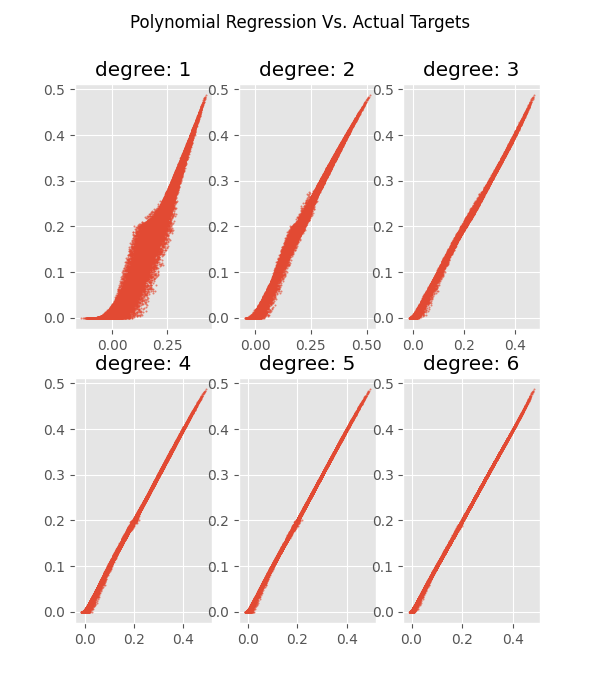
\includegraphics{Figures/polynomialEuroC.png}
\decoRule
\caption[Polynomial Regression Predictions Vs. Actual Prices]{Predicted price based on polynomial regression of varying degree}
\label{fig:PolynomialEuroC}
\end{figure}

The table is created to compare the performance for each model. The table confirms that the linear regression has a worse fit than the other models with higher capacity. The difference on the MLPs and higher order polynomial regression models less than $6\cdot 10^{-4}$ for coefficient of determination and less than $15 \cdot 10^{-3}$. The difference is negible so the fit for MLPs and polynomial regression of degree 4-6 performs all very well on the data.

\begin{table}[th]
\caption{Prediction results for european call test data for in sample polynomial regression}
\label{tab:euroPerformance}
\centering
\begin{tabular}{l l l l l l l l }
\toprule
\textbf{Model} & \textbf{Dataset} & \textbf{MSE} & \textbf{RMSE} & \textbf{MAE} & \textbf{$R^2$} \\
\midrule
Linear Reg. & In-Sample & 0.000631 & 0.025122 & 0.018264 & 0.937445\\
2. degree &  & 0.000069 & 0.008298 & 0.006136 & 0.993175\\
4. degree &  & 0.000004 & 0.002059 & 0.001282 & 0.999580\\
5. degree &  & 0.000002 & 0.001407 & 0.000864 & 0.999804\\
MLPs &  & 0.000003 & 0.001628 & 0.001337 & 0.999736\\
3. degree & In-Sample & 1.31e-05 & 0.00362470 & 0.002559 & 0.998698\\
6. degree & In-Sample & 9.23e-07 & 0.000961 & 0.000592 & 0.999908\\
MLPs & In-Sample & 0.000006 & 0.002419 & 0.001966 & 0.99942\\
\bottomrule\\
\end{tabular}
\end{table}


%-----------------------------------
%	SUBSECTION 3
%-----------------------------------
\subsection{Model Performance In-Sample}
The model performance is evaluated by MSE, RMSE, MAE and coefficient of determination, where all the measures evaluate how close is the model predictions with the actual targets. For a high quality model the first three measures should be close to 0, where the latter should be close to 1. For MSE close to 0 means that the model predictions does not differ a lot from the observed targets. The RMSE and MAE are same kind of measure, but just measured slightly different. The RMSE is the square root of MSE, which means MSE and RMSE penalize large errors. The MAE is the mean absolute error and large errors is penalized less. Coefficient of determination provides a measure of how well observed targets are replicated by the model, based on the proportion of total variation of target explained by the model.

\begin{table}[th]
\caption{Prediction results for european call test data for in sample}
\label{tab:euroParRange}
\centering
\begin{tabular}{l l l l l l }
\toprule
\textbf{MSE} & \textbf{RMSE} & \textbf{MAE} & \textbf{Coefficent of Determination} \\
\midrule
0.000006 & 0.002419 & 0.0019661242 & 0.99942\\
\bottomrule\\
\end{tabular}
\end{table}

The performance measures are generally good, we see MAE, MSE and RMSE all have values less than 0.002419 from zero and a coefficient of determination 0.00058 from 1. 

\begin{figure}[th]
\centering
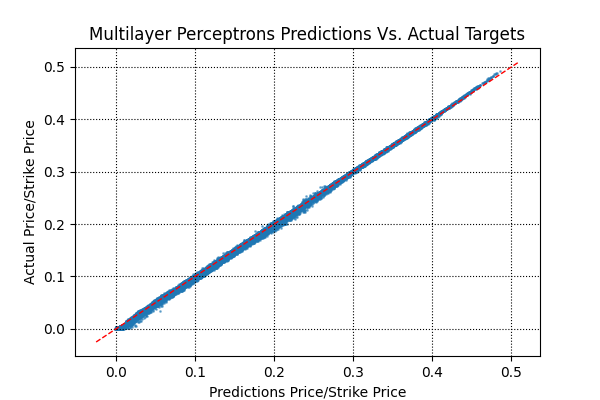
\includegraphics{Figures/PredictionEuroC.png}
\decoRule
\caption[MLPs Predictions Vs. Actual Prices]{Predicted price based on MLPs model}
\label{fig:MLPsEuroC}
\end{figure}

Illustration of the model fit is also provided, where the plot shows $\frac{c(S_0,K)}{K}$ predicted from the model and observed target values. The conclusion from the performance metrics is also present in the figure, where we see the model predicts close to target values over the whole range. Before moving on to pricing for american options, we investigate if polynomial regression can perform as MLPs



\subsection{Out of sample predictions}
All the models considered had good performance on the in-sample dataset except of the too simple models linear regression and 2. degree polynomial regreesion. To test the predictive strength for the models, we test the models with out-of-sample data. Specifically we consider longer maturity and deep-out-of-money options (see table \ref{tab:totalEuroParRange})
\begin{table}[H]
\caption{Parameter range}
\label{tab:totalEuroParRange}
\centering
\begin{tabular}{l l l l l l l }
\toprule
\textbf{Dataset} & \textbf{Moneyness} & \textbf{r} & \textbf{$\sigma$} & \textbf{T} \\
\midrule
In-Sample & 0.8-1.2 & 1\%-3\% & 0.05-0.5 & 1/252-3.0\\ 
Out-Of-Money & 0.6-0.8 & 1\%-3\% & 0.05-0.5 & 1/252-3.0\\ 
Longer Maturity & 0.8-1.2 & 1\%-3\% & 0.05-0.5 & 3-0-5.0\\ 
\bottomrule\\
\end{tabular}
\end{table}
The performance measures show that the polynomial regression that was performing better on the In-Sample dataset was due to overfitting, because the high order polynomial regression does perform poorly on out-of-sample data (see table \ref{tab:euroPerformanceComparision} and figure \ref{fig:PolynomialOutMoneyEuroC}). For the 5. order polynomial regression, we see a negative coefficient of determination, which means the model performs worse than the model with the mean as a horizontal line. This means the 5. order polynomial clearly have low predictive strength. 

\begin{table}[H]
\caption{Performance of predictive strength for different regression models}
\label{tab:euroPerformanceComparision}
\centering
\begin{tabular}{l l l l l l l l }
\toprule
\textbf{Model} & \textbf{Dataset} & \textbf{MSE} & \textbf{RMSE} & \textbf{MAE} & \textbf{$R^2$} \\
\midrule
Linear Reg. & In-Sample & 0.000631 & 0.025122 & 0.018264 & 0.937445\\
2. degree &  & 0.000069 & 0.008298 & 0.006136 & 0.993175\\
4. degree &  & 0.000004 & 0.002059 & 0.001282 & 0.999580\\
5. degree &  & 0.000002 & 0.001407 & 0.000864 & 0.999804\\
MLPs &  & 0.000003 & 0.001628 & 0.001337 & 0.999736\\
Linear Reg. & Out-Of-Money & 0.005772 & 0.075973 & 0.060936 & -2.377251\\
2. degree &  & 0.000767 & 0.027694 & 0.022203 & 0.551246\\
4. degree &  & 0.000944 & 0.030724 & 0.020542 & 0.447668\\
5. degree &  & 0.001812 & 0.042568 & 0.027125 & -0.060261\\
MLPs &  & 0.000005 & 0.002152 & 0.001569 & 0.997291\\
Linear Reg. & Longer Maturity & 0.002662 & 0.051593 & 0.041232 & 0.818143\\
2. degree &  & 0.001196 & 0.034577 & 0.026287 & 0.918316\\
4. degree &  & 0.003956 & 0.062894 & 0.039932 & 0.729744\\
5. degree &  & 0.012255 & 0.110702 & 0.064402 & 0.162742\\
MLPs &  & 0.000066 & 0.008138 & 0.005817 & 0.995475\\
\bottomrule\\
\end{tabular}
\end{table}

We see that the 2. degree polynomial is best on most of the performance measures for our-of-sample data. Notice based on MAE for out-of-money data the 4. degree polynomial performs better than the 2. degree polynomial, but if we look at the MSE the performance is best for the 2. degree polynomial. This is due to that the two measure weight errors in different ways, where the MSE penalize large error more than the MAE. Amoung the polynomial the 2. degree polynoial regression performs best, but gets outperformed by MLPs (see also figure \ref{fig:MLPsOutMoneyEuroC}). The MLPs has high predictive strength compared to the polynomials, because it performs well also on out-of-sample dataset. The section showed how succesfully MLPs can be used in a GBM model setup for pricing european options. The MLPs is not based on a model, it can only see data. This is promising because the MLPs could also be used for actual market data or different models to learn patterns. In the coming sections we will focus on american put options and basket options, where in the basket option case the MLPs benefit for the fact that it does not increase expontially with the dimension to maintain low error compared to polynomial regression. For the american put option the MLPs regression will only be considered, because the polynomial regression have low predictive strength for the simpler european option.

\begin{figure}[H]
\centering
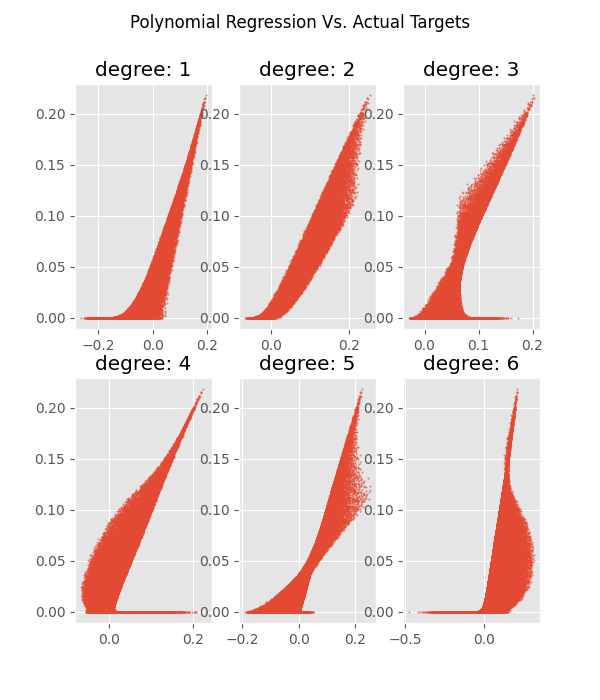
\includegraphics{Figures/polynomialOutMoneyEuroC.png}
\decoRule
\caption[Polynomial Regression Predictions Vs. Actual Prices]{Predicted price based on polynomial regression of varying degree}
\label{fig:PolynomialOutMoneyEuroC}
\end{figure}

\begin{figure}[H]
\centering
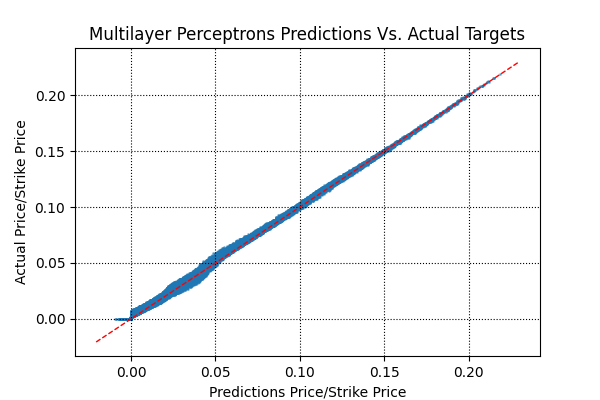
\includegraphics{Figures/PredictionOutMoneyEuroC.png}
\decoRule
\caption[MLPs Predictions Vs. Actual Prices]{Predicted price based on MLPs model}
\label{fig:MLPsOutMoneyEuroC}
\end{figure}

%\begin{figure}[th]
%\centering
%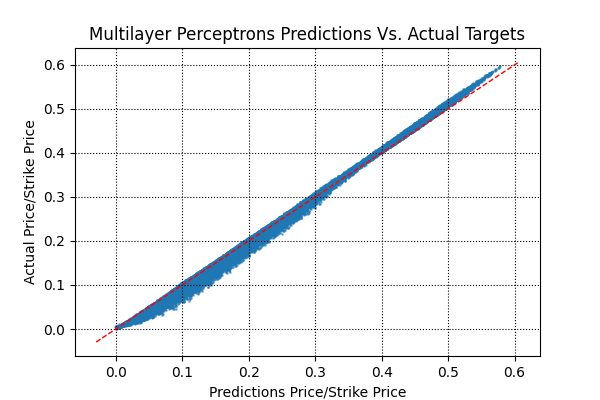
\includegraphics{Figures/PredictionLongTEuroC.png}
%\decoRule
%\caption[MLPs Predictions Vs. Actual Prices]{Predicted price based on MLPs model}
%\label{fig:MLPsEuroC}
%\end{figure}


%\begin{figure}[H]
%\centering
%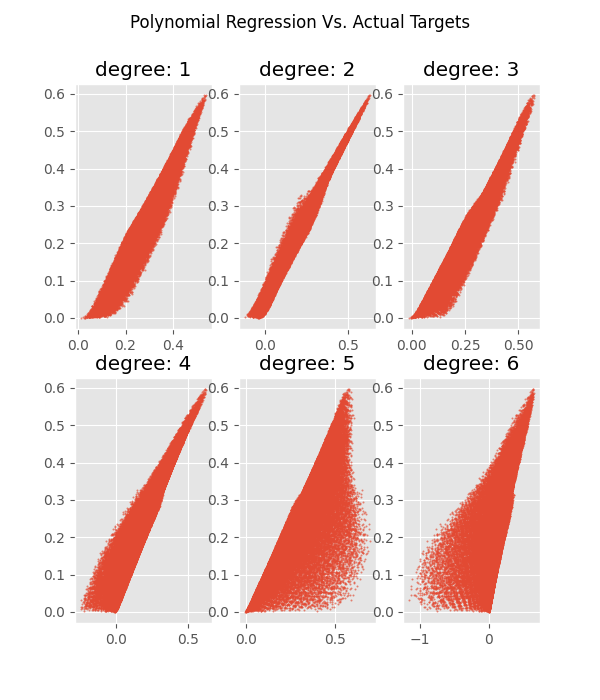
\includegraphics{Figures/polynomialLongTEuroC.png}
%\decoRule
%\caption[Polynomial Regression Predictions Vs. Actual Prices]{Predicted price based on polynomial regression of varying degree}
%\label{fig:PolynomialEuroC}
%\end{figure}


%----------------------------------------------------------------------------------------
%	SECTION 2
%----------------------------------------------------------------------------------------
\section{Multilayer Perceptrons Regression For American Options}

%-----------------------------------
%	SUBSECTION 1
%-----------------------------------
\subsection{Data}



%-----------------------------------
%	SUBSECTION 2
%-----------------------------------
\subsection{Optimization and cost function}

%-----------------------------------
%	SUBSECTION 3
%-----------------------------------
\subsection{Model Performance}

\begin{table}[H]
\caption{Performance of predictive strength for different regression models}
\label{tab:euroPerformanceComparision}
\centering
\begin{tabular}{l l l l l l l l }
\toprule
\textbf{Model} & \textbf{Dataset} & \textbf{MSE} & \textbf{RMSE} & \textbf{MAE} & \textbf{$R^2$} \\
\midrule
MLPs Reg. & In-Sample & 0.000002 & 0.001562 & 0.001278 & 0.999634\\
MLPs Reg. & Out-Of-Money & 0.000030 & 0.005503 & 0.003925 & 0.989674\\
MLPs Reg. & Longer Maturity & 0.000194 & 0.013922 & 0.010731 & 0.980759\\
\bottomrule\\
\end{tabular}
\end{table}

\begin{figure}[H]
\centering
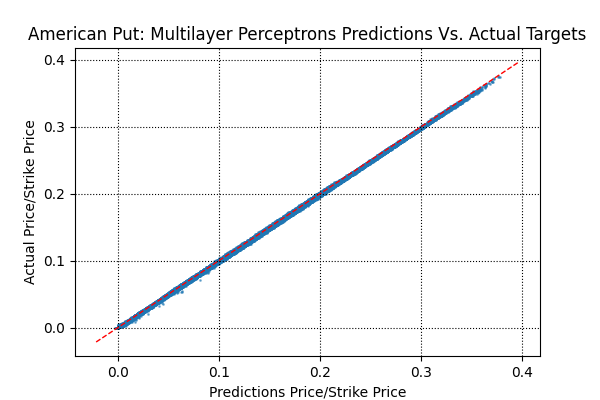
\includegraphics{Figures/PredictionAmerP.png}
\decoRule
\caption[MLPs Predictions Vs. Actual Prices For American Put]{Predicted price based on MLPs model, where the targets are from the binomial model}
\label{fig:PredictionAmerP}
\end{figure}

\begin{figure}[H]
\centering
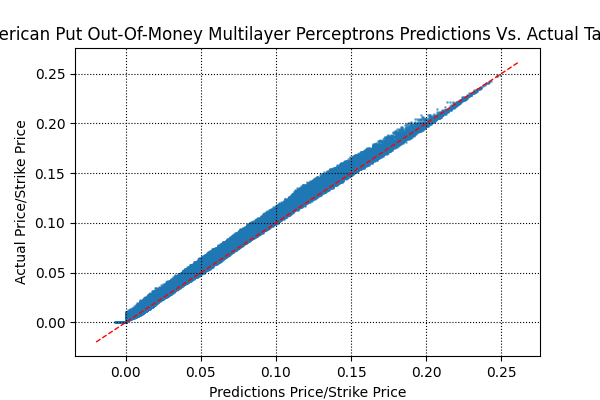
\includegraphics{Figures/PredictionOutMoneyAmerP.png}
\decoRule
\caption[MLPs Predictions Vs. Actual Prices For American Put]{Predicted price based on MLPs model, where the targets are from the binomial model}
\label{fig:PredictionOutMoneyAmerP}
\end{figure}

\begin{figure}[H]
\centering
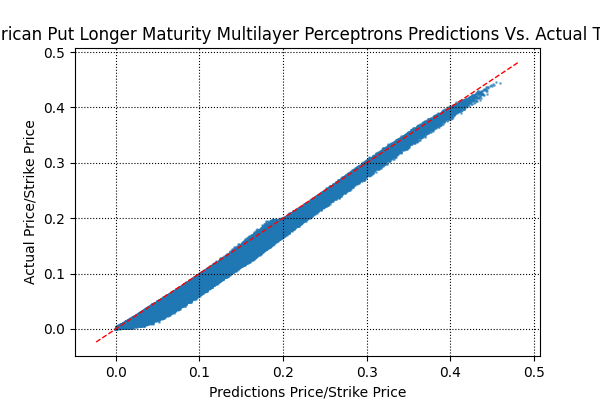
\includegraphics{Figures/PredictionLongTAmerP.png}
\decoRule
\caption[MLPs Predictions Vs. Actual Prices For American Put]{Predicted price based on MLPs model, where the targets are from the binomial model}
\label{fig:PredictionOutMoneyAmerP}
\end{figure}

To compare the results by 

\begin{table}[th]
\caption{Valuation of American put option with K=40 and r=0.06.}
\label{tab:treatments}
\centering
\begin{tabular}{l l l l l l l }
\toprule
\textbf{Spot} & \textbf{$\sigma$} & \textbf{T} & \textbf{MLPs Regression} & \textbf{Binomial Tree} & \textbf{LSM} & \textbf{abs. diff.} \\
\midrule
36 & 0.2 & 1 & 4.584 & 4.488 & 4.478 & 0.010\\
36 & 0.2 & 2 & 4.649 & 4.846 & 4.828 & 0.018\\
36 & 0.4 & 1 & 7.090 & 7.119 & 7.092 & 0.027\\
36 & 0.4 & 2 & 8.487 & 8.508 & 8.500 & 0.008\\
38 & 0.2 & 1 & 3.094 & 3.260 & 3.245 & 0.015\\
38 & 0.2 & 2 & 3.638 & 3.748 & 3.735 & 0.013\\
38 & 0.4 & 1 & 6.172 & 6.165 & 6.144 & 0.021\\
38 & 0.4 & 2 & 7.605 & 7.689 & 7.665 & 0.024\\
40 & 0.2 & 1 & 2.114 & 2.316 & 2.313 & 0.003\\
40 & 0.2 & 2 & 2.779 & 2.885 & 2.881 & 0.004\\
40 & 0.4 & 1 & 5.274 & 5.310 & 5.326 & 0.016\\
40 & 0.4 & 2 & 6.839 & 6.914 & 6.908 & 0.006\\
42 & 0.2 & 1 & 1.494 & 1.622 & 1.622 & 0.000\\
42 & 0.2 & 2 & 2.167 & 2.217 & 2.212 & 0.005\\
42 & 0.4 & 1 & 4.548 & 4.602 & 4.596 & 0.006\\
42 & 0.4 & 2 & 6.197 & 6.264 & 6.243 & 0.021\\
44 & 0.2 & 1 & 1.000 & 1.117 & 1.113 & 0.004\\
44 & 0.2 & 2 & 1.678 & 1.697 & 1.688 & 0.009\\
44 & 0.4 & 1 & 3.949 & 3.956 & 3.962 & 0.006\\
44 & 0.4 & 2 & 5.649 & 5.656 & 5.649 & 0.007\\
\bottomrule\\
\end{tabular}
\end{table}


The results are promosing, because the MLPs are model free in the sense, that we could have simulated out for any model, where MLPs then learn from data only. By observing this the method can be extended to real market data in fact \parencite{GasparRaquel20} have resently showed good results for a MLPs for real market data. The next section will investigate the curse of dimensionality and the application of MLPs in this context.
\parencite{FergusonRyan2018}









